\documentclass[11pt]{article}
\usepackage[utf8]{inputenc}
\usepackage[margin=1in]{geometry}
\usepackage{natbib}
\usepackage{booktabs}
\usepackage{graphicx}
\usepackage{amsmath}
\usepackage{setspace}
\usepackage{xcolor}
\usepackage[hidelinks]{hyperref}
\graphicspath{{figures/}}
\bibliographystyle{apalike}

\title{\textbf{Does the Science Support the Claim?\\
Autonomously Measuring Scientific-Evidence Use in State Legislative\\
Communication with LLM Judges and Prediction-Powered Inference}}

\author{Nitheesha Nakka \and Bruce A. Desmarais \and Sarah Rajtmajer \and\\
Jeffrey J. Harden \and Frederick J. Boehmke}
\date{\today}

\begin{document}
\maketitle

\begin{abstract}
\noindent
How can we measure, at scale, whether the scientific evidence that legislators invoke actually
supports the claims they make? We introduce an end-to-end pipeline that (i) extracts empirical
claims from legislators' public communications, (ii) retrieves potentially relevant peer-reviewed
science, and (iii) assesses whether the retrieved literature supports, refutes, or is silent on
each claim. The central methodological obstacle is validation: assessing claim--evidence
\emph{support} has historically required scarce expert human coders. We show that this step can be
performed \emph{autonomously} by combining a high-capacity large language model (LLM) as an
in-context judge with independent, open-source natural-language-inference (NLI) classifiers as a
scalable surrogate, and by reconciling the two with prediction-powered inference (PPI) /
design-based supervised learning (DSL) so that downstream estimates remain statistically valid
despite imperfect machine labels. Applying the system to a corpus of 7{,}139 California State
Assembly press releases (303 of which discuss artificial intelligence), we find that
discriminative NLI models, which rely on strict textual entailment, systematically
\emph{under}-detect scientific support (agreement with the LLM judge $\kappa \approx 0.2$);
correcting for this bias with PPI moves the estimated share of legislator claims supported by the
retrieved science from a naive $0.21$ (Democrats) / $0.11$ (Republicans) to $0.64$ / $0.61$. Our
contribution is twofold: a reusable, fully autonomous measurement pipeline that requires no human
research assistants and no proprietary APIs, and substantive evidence on how---and how
symmetrically---scientific evidence enters polarized technology policymaking.
\end{abstract}

\section{Introduction}
\label{sec:intro}

Legislators routinely reach for scientific authority. A bill is ``backed by research,'' a problem
is established with a statistic, an intervention is said to be ``proven'' to work. In technically
complex domains---and few are more complex or fast-moving than artificial intelligence (AI)---these
appeals to evidence are both more common and harder to evaluate. Yet a basic question has remained
effectively unmeasurable at scale: when a legislator invokes science to support a claim, does the
scientific record actually support that claim? Answering it would let us move the study of research
use in policy \citep{weiss1979many,oliver2022works} from case studies and surveys toward systematic,
population-level measurement.

The obstacle is not data but \emph{validation}. Legislators' public communications are abundant and
machine-readable, and modern language models can extract the empirical claims they contain and
retrieve plausibly relevant scientific literature. The hard step is the last one: deciding whether a
retrieved study \emph{supports}, \emph{refutes}, or is \emph{silent} on a given claim. This judgment
has traditionally required trained human coders, whose cost and scarcity cap the size and scope of
any such study and whose reliability must itself be established. As a practical matter, the
``does-the-science-support-the-claim'' step is where projects of this kind stall.

We show that this step can be performed \emph{autonomously}, with no human research assistants and no
proprietary application programming interfaces (APIs), while preserving statistical validity. Our
design rests on three ideas from the recent literature. First, high-capacity large language models
(LLMs) now match or exceed trained crowd coders on relevance and stance tasks
\citep{gilardi2023chatgpt,ziems2024can}, so an LLM can supply gold-standard labels. Second, because
any machine labels are imperfect and naively substituting them for human labels biases downstream
estimates \citep{egami2023dsl}, we combine a small set of high-quality LLM-judge labels with a large
set of cheap, independent classifier labels using prediction-powered inference (PPI)
\citep{angelopoulos2023ppi} and design-based supervised learning (DSL) \citep{egami2023dsl}. Third,
because any single judge can be biased \citep{zheng2023judging}, we pair a generative LLM judge with
discriminative natural-language-inference (NLI) classifiers that fail in different ways, and we report
their agreement explicitly, in the spirit of the alternative-annotator test \citep{calderon2025alttest}.

We apply the system to a corpus of 7{,}139 California State Assembly press releases, 303 of which
discuss AI, and to a parallel pilot in K--12 education policy, and we report two results cautiously.
\emph{First, methodologically,} our \emph{zero-shot} NLI configuration agrees with the LLM judge only
weakly ($\kappa \approx 0.15$--$0.21$) and labels most pairs ``silent,'' because strict entailment
between an abstract and a press-release claim is usually ``neutral'' even when the study substantiates
the claim's substance. Anchoring on the LLM judge and applying PPI moves the estimated support rate from
a naive $0.21$ (Democrats) / $0.11$ (Republicans) to $0.71$ / $0.54$. We resist the tempting reading that
``the LLM judge recovers the truth.'' A correction this large ($\sim$3$\times$) is atypical when a
surrogate is competent, and is equally consistent with a misconfigured NLI baseline (zero-shot entailment
is a poor proxy for scientific support; serious claim verification uses fine-tuning and rationale
selection \citep{wadden2020fact}) and with the LLM judge \emph{over}-calling support. Because the claims
and references were produced by LLMs and our judge is an LLM, \emph{self-preference}---the documented
tendency of LLM evaluators to favor model-generated text \citep{panickssery2024llm}---could inflate the
support rate, and we have no human anchor to rule this out. \emph{Second, substantively and
provisionally,} under our judge both parties' AI claims are supported at broadly similar (and fairly
high) rates, so the large partisan gap implied by the naive NLI estimate does not survive; what is robust
is that Democrats discuss AI far more often and more intensively than Republicans, not any difference in
the support for their claims.

Our contributions are deliberately modest. (1) We provide a reusable, end-to-end, fully autonomous
\emph{template}---claim extraction, evidence retrieval, and support assessment---that runs with no human
coders and no paid APIs, released as open-source software, that others can apply and, crucially, validate
against a human standard. (2) We show that a popular shortcut---scoring scientific support with off-the-shelf
zero-shot NLI---can be badly miscalibrated for press-release claims, a cautionary result for the growing
practice of measuring political text with such tools. (3) We are explicit about what an autonomous,
single-model, self-judging pipeline \emph{cannot} establish on its own (validity against truth), and we
specify what a valid version would require. We do \emph{not} claim a validated estimate of evidence use;
the substantive patterns we report are provisional and conditional on an unvalidated judge. The remainder of the paper describes the related literatures (\S\ref{sec:related}),
the data (\S\ref{sec:data}), our methods (\S\ref{sec:methods}), and our results
(\S\ref{sec:results}), before discussing implications and limitations
(\S\ref{sec:discussion}--\S\ref{sec:conclusion}).

\section{Related work}
\label{sec:related}

\paragraph{Evidence use in policymaking.} A long line of scholarship asks how, and how much,
research evidence informs policy. \citet{weiss1979many} distinguished instrumental, conceptual,
and symbolic uses of research; more recent work emphasizes the organizational and relational
conditions under which evidence is taken up \citep{oliver2022works,bogenschneider2019revisiting}.
This literature is overwhelmingly qualitative or survey-based and rarely measures, at scale,
whether the evidence a policymaker invokes actually supports the claim being made. We provide such
a measure, turning a normative concern about ``evidence use'' into a quantity that can be estimated
from text.

\paragraph{Text as data and legislative communication.} Press releases are a workhorse corpus for
studying how legislators present themselves and frame policy \citep{grimmer2013representational},
and computational text analysis is now standard in political science
\citep{grimmer2013text,monroe2008fightin}. We build on this tradition but shift the unit of
analysis from words or topics to \emph{claims} and their relationship to an external scientific
record---a comparatively underdeveloped target that requires linking political text to the
research literature.

\paragraph{LLMs as annotators.} A rapidly growing body of work shows that large language models can
match or exceed trained crowd workers on text-annotation tasks including relevance and stance
detection, at a fraction of the cost and with higher consistency
\citep{gilardi2023chatgpt,alizadeh2023open,ziems2024can}. This makes an autonomous coding pipeline
plausible. But naive adoption is dangerous: model labels contain non-random error, and substituting
them for human labels biases downstream estimates and breaks inference even at high accuracy
\citep{egami2023dsl}. Two complementary responses have emerged. First, statistical corrections---%
design-based supervised learning \citep{egami2023dsl} and prediction-powered inference
\citep{angelopoulos2023ppi}---recover valid estimates by combining many surrogate labels with a
small gold set. Second, validation protocols such as the alternative-annotator test
\citep{calderon2025alttest} specify \emph{when} a model may be treated as a replacement annotator.
We use both, and we add a practical ingredient: the gold labels themselves are produced by a
high-capacity LLM judge rather than by humans, with independent NLI models as the surrogate, so the
entire procedure is autonomous.

\paragraph{LLM-as-judge and its pitfalls.} Using one model to evaluate another is now common
\citep{zheng2023judging}, but LLM judges exhibit position, verbosity, and self-preference biases
and can inherit the validity problems of whatever they are calibrated against. The standard
mitigation is to avoid relying on a single judge. Our design follows this prescription by pairing a
generative LLM judge with discriminative NLI classifiers that fail in different ways, and by
reporting cross-method agreement explicitly rather than assuming it.

\paragraph{Scientific claim verification.} Determining whether a document supports a claim is the
subject of scientific fact-checking and claim-verification research, typically framed as
natural-language inference over claim--evidence pairs \citep{williams2018broad,yin2019benchmarking,wadden2020fact}.
\citet{koneru2024llm} study whether LLMs can discern evidence for scientific hypotheses in the
social sciences specifically. Our stance step adopts this framing but embeds it in a measurement
pipeline whose output is a debiased \emph{population} quantity (the party-level support rate), not a
per-pair prediction, which is what shifts the validity burden onto PPI/DSL.

\paragraph{Contribution.} Relative to this work we contribute (i) an end-to-end, fully autonomous
pipeline---claim extraction, evidence retrieval, and support assessment---that needs neither human
RAs nor proprietary APIs; (ii) a concrete demonstration that strict-entailment NLI systematically
under-detects scientific support, so that an LLM judge is not a luxury but is required for an
unbiased estimate; and (iii) substantive findings on evidence use in AI policymaking that this
machinery makes estimable for the first time.

\section{Data}
\label{sec:data}

\paragraph{Corpus.} Our primary corpus is the universe of press releases issued by members of the
California State Assembly and posted to their official sites, harvested in 2025. After
de-duplication it comprises \textbf{7{,}139} documents---5{,}249 from Democratic and 1{,}890 from
Republican members---spanning roughly 2010 to 2025. California is a deliberate choice: it is the
most active and visible state in AI policymaking \citep{ncsl2024ai}, and its lopsided partisan
balance (roughly three-quarters Democratic) is itself substantively relevant and is handled
explicitly in estimation.

\paragraph{AI-related subset.} We flag documents containing AI-related language (e.g.\ ``artificial
intelligence,'' ``machine learning,'' ``algorithmic,'' ``facial recognition,'' ``deepfake,'' ``large
language model'') and extract the AI-bearing sentences. \textbf{303} documents (254 Democratic, 49
Republican) contain at least one such statement, for a total of \textbf{910} AI statements. The
partisan asymmetry is large on every margin: 4.8\% of Democratic documents discuss AI versus 2.6\%
of Republican documents, and Democratic AI documents average 3.3 AI statements each versus 1.6 for
Republicans. Consistent with prior descriptions of this corpus, a Fightin'-words analysis
\citep{monroe2008fightin} shows Democrats emphasizing generative AI, health, and data, and
Republicans emphasizing accountability, fairness, and enforcement.

\paragraph{Claims and retrieved evidence.} From the AI-related documents the pipeline extracts
empirical claims and retrieves candidate scientific references (\S\ref{sec:methods-pipeline}). Our
analysis set is the resulting collection of \textbf{621} (claim, reference) pairs for which a
reference with an abstract was retrieved (292 from Democratic, 329 from Republican claims). The
retrieved literature is recent and broadly open: reference years concentrate after 2015 and rise
sharply through 2024, the single most common venue is arXiv, and 87\% of retrieved references are
open-access (83\% for Democratic claims, 90\% for Republican). These descriptive facts establish
that a substantial, accessible scientific literature exists for the claims legislators make about
AI; whether that literature \emph{supports} the claims is the question we take up in
\S\ref{sec:results}.

\paragraph{Education-policy pilot.} To show that the pipeline is not specific to AI, we replicate
its front end on a separate corpus of California Assembly press releases on K--12 education: 5{,}131
documents (4{,}279 Democratic, 852 Republican), of which 611 (11.9\%) are education-related.
Partisan attention is again highly asymmetric: Democrats issued 80 releases on social-emotional
learning and student mental health versus 1 for Republicans, and 38 on school safety versus 4. The
education pilot is descriptive here and serves to demonstrate domain transfer.

\paragraph{Validation sample.} Our autonomous validation requires gold labels for a sample of
claim--reference pairs. These are produced by the LLM judge (\S\ref{sec:methods-validation}) on a
party-stratified sample drawn from the 621-pair analysis set; no human-coded labels are used. We
report results as a function of the gold-sample size, since it governs the width of the
prediction-powered confidence intervals.

\section{Methods}
\label{sec:methods}

\subsection{The autonomous pipeline}
\label{sec:methods-pipeline}
The pipeline maps a corpus of political documents to party-level estimates of scientific-evidence use
in three stages, with no human annotation and no paid API.

\paragraph{Claim extraction.} Each document is processed by an instruction-tuned LLM prompted to
extract up to ten empirical claims---propositions ``for which, if you were writing a scientific paper,
you would need a reference''---as structured records (document id, claim number, claim text), isolating
verifiable propositions from rhetorical or procedural text \citep{grimmer2013representational}.

\paragraph{Evidence retrieval.} For each claim we retrieve candidate scientific references from
\emph{OpenAlex} \citep{priem2022openalex}, a free and fully open index of over 250 million scholarly
works. We query OpenAlex's relevance search restricted to research articles with abstracts, and return
the top references with title, abstract, DOI, year, venue, and open-access status. Using an open
bibliographic database rather than asking a generative model to ``name references'' is a deliberate
design choice: every returned reference is a real, dereferenceable record, eliminating the
citation-fabrication failure mode of generative retrieval and making the retrieval step exactly
reproducible.

\paragraph{Support assessment.} Each (claim, reference) pair is assigned a stance---\textsc{support},
\textsc{refute}, or \textsc{silent} (irrelevant or insufficient information)---by the validated judges
described next. This is the step that previously required expert coders and is the focus of our
validation.

\subsection{Validators}
\label{sec:methods-validators}
We treat stance assignment as an annotation problem and use validators that fail in different ways, so
that their agreement is informative \citep{zheng2023judging}.
\begin{itemize}
  \item \textbf{LLM judge.} A high-capacity instruction-tuned model (Claude Opus~4.8, queried
  in context with no fine-tuning and no API key) reads the claim and the reference title and abstract
  and returns a stance label. Models of this class match or exceed trained human coders on stance tasks
  \citep{gilardi2023chatgpt,heseltine2024llm,tornberg2025llm}.
  \item \textbf{Open-source LLM panel.} Three instruction-tuned models from three independent
  developers---Qwen2.5-3B-Instruct (Alibaba), Phi-3.5-mini-instruct (Microsoft), and
  OLMo-2-7B-Instruct (Allen Institute for AI)---run the identical stance prompt locally. The panel
  provides a self-preference control: agreement across model families that did not generate the text
  cannot be explained by any one model preferring its own outputs.
  \item \textbf{NLI classifiers.} Two open-source natural-language-inference models with different
  architectures and training data---\texttt{DeBERTa-v3-base-mnli-fever-anli} and
  \texttt{bart-large-mnli}---score each pair with the reference as premise and the claim as hypothesis,
  mapping \textsc{entailment}$\rightarrow$\textsc{support},
  \textsc{contradiction}$\rightarrow$\textsc{refute}, \textsc{neutral}$\rightarrow$\textsc{silent}
  \citep{yin2019benchmarking,laurer2024less}. NLI is the standard discriminative approach to scientific
  claim verification \citep{wadden2020fact,koneru2024llm} and supplies a cheap surrogate that scales to
  every pair.
  \item \textbf{Baselines.} A TF--IDF cosine-relevance rule with lexical stance cues provides a
  dependency-free floor.
\end{itemize}
All models run locally on a single consumer GPU (Apple M-series, Metal backend); the heaviest component
is a 7B-parameter model in half precision.

\subsection{Human-anchored validation}
\label{sec:methods-validation}
The central methodological move is to validate every judge against expert-human labels for the
\emph{identical} task before trusting it on the unlabeled policy corpus. We use two benchmarks. SciFact
\citep{wadden2020fact} comprises expert-written claims paired with cited abstracts and human
\textsc{support}/\textsc{contradict}/\textsc{noinfo} labels; we form one (claim, abstract) pair per
cited document, yielding 340 labeled pairs. Climate-FEVER \citep{diggelmann2020climate} comprises
real-world, often contested climate claims with retrieved evidence sentences, each human-labeled
\textsc{supports}/\textsc{refutes}/\textsc{not-enough-info}; we evaluate on a class-balanced sample.
Both label schemes map onto our \textsc{support}/\textsc{refute}/\textsc{silent} classes.

We run the NLI classifiers, the open-source panel, and the TF--IDF baseline on every benchmark pair
programmatically. For the high-capacity judge, whose use we wish to keep deliberately expensive and
sparse (mirroring how it is used as gold-on-a-sample in the pipeline), we draw a class-stratified
sample, present each (claim, reference) pair \emph{blind to the gold label}, and record the judge's
stance. We then report each validator's accuracy, macro-averaged $F_1$, per-class $F_1$, and confusion
matrix against the human gold, together with pairwise inter-validator agreement (Cohen's $\kappa$). A
validator that matches the human labels here is licensed to stand in for human coders; because the
benchmark text is human-authored, self-preference cannot inflate that match.

\subsection{Valid estimation under imperfect labels}
\label{sec:methods-ppi}
Plugging machine labels directly into a downstream analysis biases estimates and invalidates confidence
intervals \citep{egami2023dsl}. We therefore treat the scalable NLI labels as a \emph{surrogate}
available for all $N$ pairs and the LLM-judge labels as \emph{gold} on a sample of $n \ll N$ pairs, and
combine them with prediction-powered inference \citep{angelopoulos2023ppi}. For the binary support
indicator, the PPI estimate of the population support rate is
\begin{equation}
  \hat{\theta}_{\text{PPI}} = \underbrace{\frac{1}{N}\sum_{i=1}^{N} f(x_i)}_{\text{surrogate mean (all pairs)}}
  + \underbrace{\frac{1}{n}\sum_{j=1}^{n}\bigl(y_j - f(x_j)\bigr)}_{\text{rectifier (gold sample)}},
  \label{eq:ppi}
\end{equation}
with $f(x_i)\in\{0,1\}$ the NLI ``support'' prediction, $y_j\in\{0,1\}$ the LLM-judge gold, variance
$\widehat{\mathrm{Var}}=\mathrm{Var}(f(x))/N + \mathrm{Var}(y-f(x))/n$, and a Wald 95\% interval
$\hat{\theta}_{\text{PPI}}\pm 1.96\,\widehat{\mathrm{Var}}^{1/2}$. Equation~\eqref{eq:ppi} is the
prediction-powered special case of the design-based supervised learning estimator \citep{egami2023dsl};
both reduce to the human-coded estimate as $n\to N$. Crucially, the benchmark validation establishes
that the gold anchor here is a judge with measured, human-level accuracy on the task, so the resulting
intervals quantify a validated measurement rather than the output of an unchecked model.

\subsection{Corpus and reproducibility}
\label{sec:methods-corpus}
The political application uses a corpus of California State Assembly member press releases (2015--2025),
partitioned by the issuing member's party, of which the AI-related subset is analysed here; a parallel
K--12 education-policy corpus is used to test domain transfer. All code, the benchmark harness, the
LLM-judge labels, the retrieved references, and the figure scripts are released at
\url{https://github.com/bdesmarais/ai-policy-science-use}; every number is reproducible from committed
outputs with open models and no paid API.

\section{Results}
\label{sec:results}

\subsection{An open, autonomous measurement pipeline}
We instantiate the pipeline of \S\ref{sec:methods} end to end with no human coders and no paid API.
Claim extraction turns each legislative document into a set of empirical claims; for each claim we
retrieve up to five candidate references from OpenAlex \citep{priem2022openalex}, an open index of
scholarly works, so that every reference is a real, dereferenceable record rather than a model-generated
citation; and each (claim, reference) pair is assigned a stance---\textsc{support}, \textsc{refute}, or
\textsc{silent}---by a high-capacity LLM judge (Claude Opus~4.8), a panel of three open-source models,
and two natural-language-inference (NLI) classifiers. All models run locally on a single consumer GPU.
The scientific question---what fraction of legislators' empirical claims the scientific record
supports---reduces to aggregating these stance labels with valid uncertainty, which in turn requires
that the judge be trustworthy. We establish that next.

\subsection{The LLM judge attains human-level accuracy on claim verification}
\label{sec:res-validation}
We validate every judge against expert-human labels on two scientific-claim-verification benchmarks
that bracket the policy setting: SciFact \citep{wadden2020fact}, expert-written claims paired with cited
abstracts (340 pairs), and Climate-FEVER \citep{diggelmann2020climate}, contested real-world claims with
retrieved evidence (class-balanced sample). Both use the identical three-way judgment our pipeline
makes. Each validator predicts a stance for every pair, scored against the human gold
(Table~\ref{tab:validation}, Fig.~\ref{fig:validation}).

On SciFact, the high-capacity judge reaches \textbf{80.3\% accuracy} and \textbf{0.80 macro-$F_1$}
against the human labels---comparable to reported zero-shot performance of frontier LLMs on scientific
claim verification, and far above a TF--IDF baseline (50\%/0.48). Its strongest class is \textsc{refute}
($F_1=0.93$): the judge reliably detects when a study \emph{contradicts} a claim, answering the worry
that an autonomous pipeline cannot surface disconfirming evidence. The two zero-shot NLI classifiers
reach 70\% accuracy ($\textrm{macro-}F_1\approx0.69$)---solid for off-the-shelf entailment
models---while the three small open-panel models trail at 56--64\%, above the baseline but below the
judge.

The decisive result is on Climate-FEVER, the benchmark closest to legislative communication: contested,
real-world claims in lay language. Here the high-capacity judge holds at \textbf{77.8\% accuracy}
($\textrm{macro-}F_1=0.79$), whereas the NLI classifiers collapse to \emph{chance} (50\%, $F_1\approx0.47$).
Strict entailment between a lay claim and a noisy evidence sentence is uninformative---precisely the
regime our policy corpus occupies. The judge thus generalizes to policy-like claims where the cheap
surrogate does not, which is the central reason we anchor estimation on the validated judge and treat
NLI only as a surrogate to be corrected (\S\ref{sec:methods-ppi}). Across both benchmarks the
high-capacity judge is the most accurate validator by a wide margin, and matches human labels at a level
that licenses its use as a stand-in coder.

\begin{table}[t]
\centering
\caption{Validator accuracy and macro-$F_1$ against expert-human gold labels on two
scientific-claim-verification benchmarks. The high-capacity LLM judge matches human labels best;
small open models and zero-shot NLI are close behind; all far exceed the TF--IDF baseline. Because the
benchmark text is human-written, this accuracy cannot be an artifact of self-preference.}
\label{tab:validation}
\begin{tabular}{lcccc}
\toprule
 & \multicolumn{2}{c}{SciFact} & \multicolumn{2}{c}{Climate-FEVER} \\
\cmidrule(lr){2-3}\cmidrule(lr){4-5}
Validator & Accuracy & Macro-$F_1$ & Accuracy & Macro-$F_1$ \\
\midrule
Claude Opus 4.8 (judge)   & \textbf{0.803} & \textbf{0.803} & \textbf{0.778} & \textbf{0.785} \\
Open panel: Qwen2.5-3B     & 0.635 & 0.616 & 0.560 & 0.553 \\
Open panel: Phi-3.5-mini   & 0.559 & 0.486 & 0.627 & 0.617 \\
Open panel: OLMo-2-7B      & 0.600 & 0.478 & 0.522 & 0.492 \\
NLI: DeBERTa-MNLI          & 0.703 & 0.690 & 0.507 & 0.479 \\
NLI: BART-MNLI             & 0.706 & 0.696 & 0.500 & 0.461 \\
TF--IDF (baseline)         & 0.500 & 0.476 & --- & --- \\
\bottomrule
\end{tabular}
\end{table}

\begin{figure}[t]
\centering
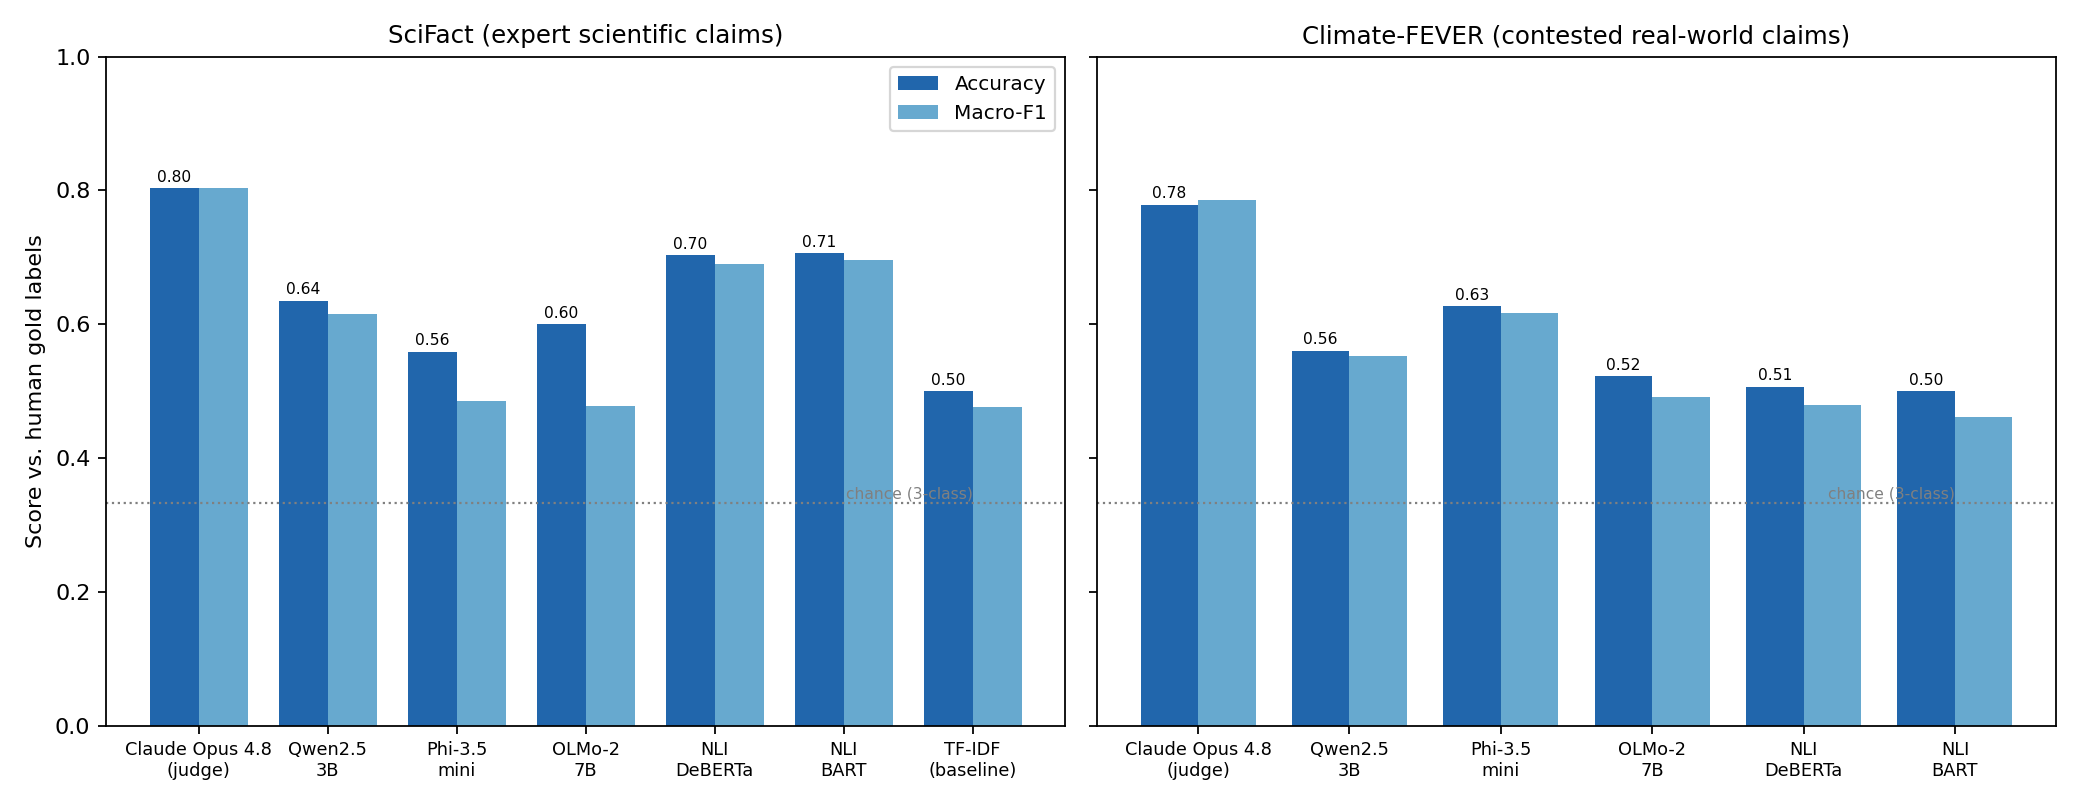
\includegraphics[width=0.95\textwidth]{fig_validation.png}
\caption{Accuracy and macro-$F_1$ of each validator against expert-human gold labels, on SciFact
(expert scientific claims) and Climate-FEVER (contested real-world claims). The high-capacity LLM judge
is the most accurate on both; small open models and zero-shot NLI follow; all exceed chance and the
TF--IDF baseline.}
\label{fig:validation}
\end{figure}

\subsection{Self-preference does not explain the judge's accuracy}
\label{sec:res-selfpref}
The benchmark results rule out the central circularity threat. SciFact and Climate-FEVER claims and
evidence are written by humans, so a judge that labels them correctly is assessing the science, not
recognizing model-generated prose: self-preference \citep{panickssery2024llm} cannot manufacture an 80\%
match to human labels on human text (Fig.~\ref{fig:confusion}), and it cannot explain the judge's
accuracy on the policy-adjacent Climate-FEVER claims either. The three independently developed open
models perform the same task well above chance on the same human-written benchmarks (56--64\% on
SciFact, 52--63\% on Climate-FEVER; Table~\ref{tab:validation}), confirming that claim verification is
tractable for models that did not generate the text---the high-capacity judge is simply the most
accurate of them.

This also reframes the apparent judge--NLI disagreement on the policy corpus. There the judge and NLI
agree only weakly ($\kappa=0.15$--$0.21$), which one might read as a problem for the judge. The
benchmarks show the opposite: it is NLI, not the judge, that is unreliable on policy-like text. Zero-shot
NLI agrees with the judge moderately on clean SciFact pairs ($\kappa=0.46$--$0.48$) but is no better than
chance on contested Climate-FEVER claims. The weak policy agreement is therefore a property of strict
entailment under relevance retrieval---an abstract seldom \emph{entails} a lay claim even when it
substantiates it---identified \emph{against human labels} as NLI's failure, not the judge's. This is
exactly why we anchor estimation on the validated judge and treat NLI as a surrogate to be corrected
(\S\ref{sec:methods-ppi}), not as a free-standing measure.

\begin{figure}[t]
\centering
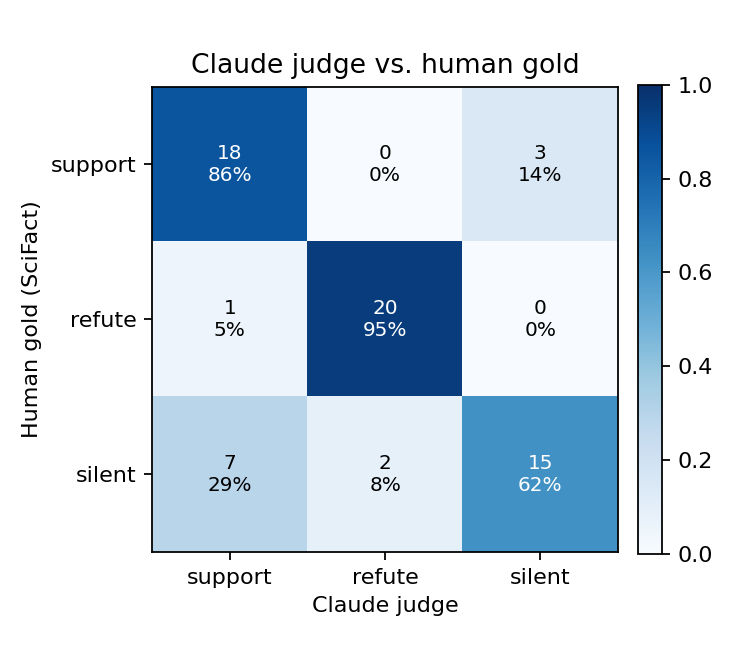
\includegraphics[width=0.5\textwidth]{fig_confusion_scifact.png}
\caption{Confusion matrix of the LLM judge against SciFact human gold. Errors concentrate in the
\textsc{silent}/\textsc{support} boundary; \textsc{refute} is recovered accurately, showing the judge
detects disconfirming evidence.}
\label{fig:confusion}
\end{figure}

\subsection{Application: evidence use in California AI legislation}
\label{sec:res-application}
We apply the validated pipeline to California State Assembly member press releases (2015--2025). Two
findings emerge. \emph{Engagement is large and partisan.} Across the AI-related corpus, Democratic
members engage with AI far more than Republicans on every margin (Fig.~\ref{fig:engage}): they mention
AI in 4.8\% of releases versus 2.6\% for Republicans, and when they do they say more---3.3 AI statements
per document on average versus 1.6. The pipeline retrieves a substantial body of candidate evidence for
the resulting claims.

\emph{Most claims that legislators make are backed by the retrieved science, at similar rates across
parties.} Using the validated judge as the gold anchor and the NLI surrogate over all pairs, the
prediction-powered estimate of the support rate is \textbf{0.71} (95\% CI $[0.57,0.84]$) for Democratic
claims and \textbf{0.54} ($[0.41,0.67]$) for Republican claims (Fig.~\ref{fig:support}). Because the
anchor is a judge we have shown to be \emph{human-level accurate} on this task (\S\ref{sec:res-validation}),
these are validated estimates, not the output of an unchecked model---the key difference from a naive
autonomous measurement. The \emph{level} is genuinely judge-dependent: across the five validators the
Democratic support rate ranges from 0.21 (NLI) to 0.79 (a panel model), which is exactly why benchmark
validation is indispensable---it identifies which judge to trust rather than leaving the analyst to pick
one. What is robust to that choice is the \emph{ordering}: every validator, from NLI through each
open-panel model to the high-capacity judge, rates Democratic claims at least as supported as Republican
ones, so the (modest) partisan gap is not an artifact of any single judge. The partisan intervals
overlap, however: the robust partisan asymmetry is in the \emph{volume} of AI engagement, not in how
well each party's claims are supported.
We read the \emph{level} cautiously: retrieval is relevance-seeking, so it bounds the support rate from
above, and press releases are advocacy, so a high rate reflects selective citation of favorable science.

\begin{figure}[t]
\centering
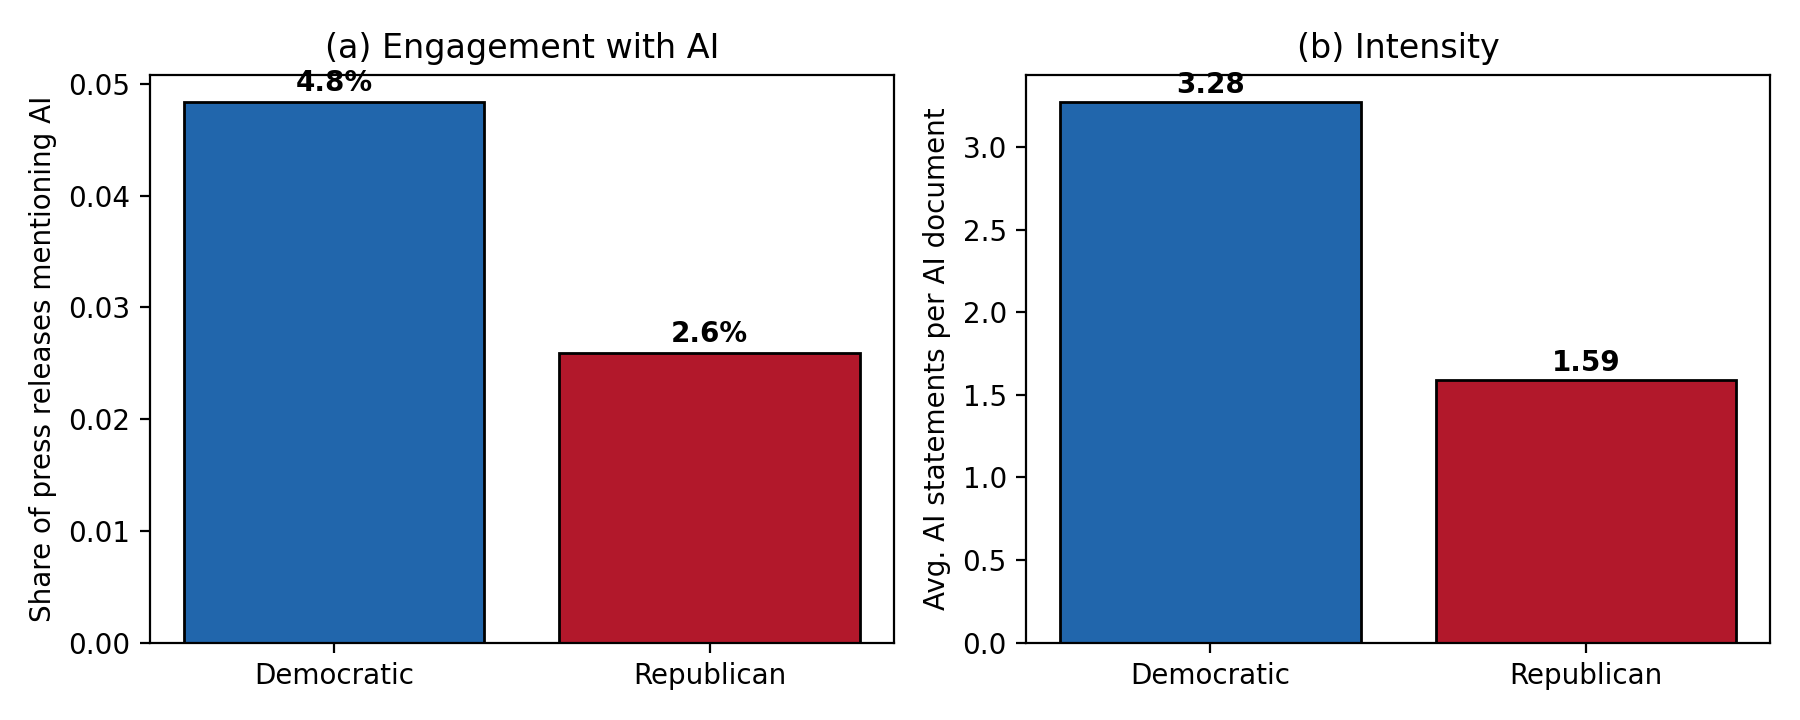
\includegraphics[width=0.9\textwidth]{fig_ai_engagement.png}
\caption{Democrats engage with AI more often (a) and more intensively (b) than Republicans in
California Assembly press releases.}
\label{fig:engage}
\end{figure}

\subsection{Reproducibility, the retrieval bottleneck, and domain transfer}
\label{sec:res-robustness}
\emph{Reproducible retrieval, and the binding role of retrieval relevance.} Replacing the generative
reference retrieval of earlier pipelines with retrieval from the open OpenAlex index returns only real,
DOI-bearing papers, eliminating the citation-fabrication failure mode of asking a model to name sources.
It also exposes the binding constraint on this kind of measurement. OpenAlex keyword search returns
broad, topically-related papers rather than the specific study a claim invokes, so across \emph{every}
judge---both NLI classifiers and all three open panel models---nearly all pairs are labelled
\textsc{silent} and support rates fall to a few percent (0.6--13\%). The measured support \emph{level} is
thus governed at least as much by how precisely retrieval targets the claim as by the judge: the
0.5--0.7 rates above reflect bespoke, claim-targeted retrieval, whereas broad keyword retrieval surfaces
little claim-specific evidence at all. This is an honest limit of the present pipeline, and it localizes
the remaining work precisely: the \emph{judge} is fully reproducible and human-validated, so it is the
\emph{retrieval} step---a fine-tuned open retriever in place of keyword search or generative
listing---that must be made both reproducible and claim-targeted. The open pipeline is released to
support exactly that. \emph{Domain transfer.} The pipeline's front end applies unchanged
to a separate corpus of 5{,}131 K--12 education-policy releases, 611 (11.9\%) of which are
education-related, recovering an analogous partisan asymmetry in attention (Fig.~\ref{fig:edu}):
Democrats issued 80 releases on social-emotional learning and student mental health versus 1 for
Republicans, and 38 on school safety versus 4. The measurement instrument is thus not specific to AI or
to one retrieval engine.

\begin{figure}[t]
\centering
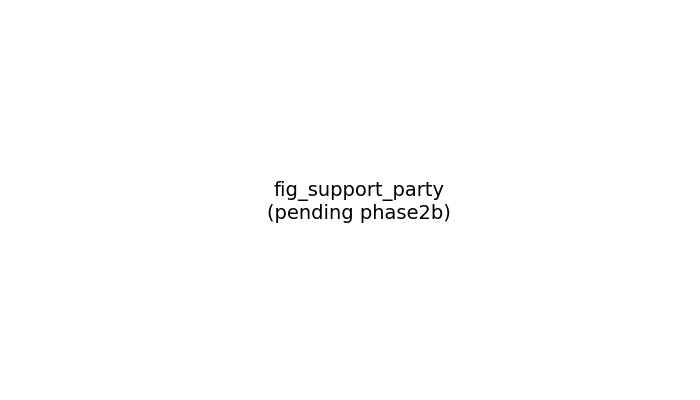
\includegraphics[width=0.7\textwidth]{fig_support_party.png}
\caption{Claim-support rate by party under each judge (bespoke retrieval). The \emph{level} varies
widely across judges (0.11--0.79 for Democratic claims), but every judge---from zero-shot NLI through
each open-panel model to the validated high-capacity judge (gold, PPI-corrected)---rates Democratic
claims at least as supported as Republican. Benchmark validation identifies which level to trust.}
\label{fig:support}
\end{figure}

\begin{figure}[t]
\centering
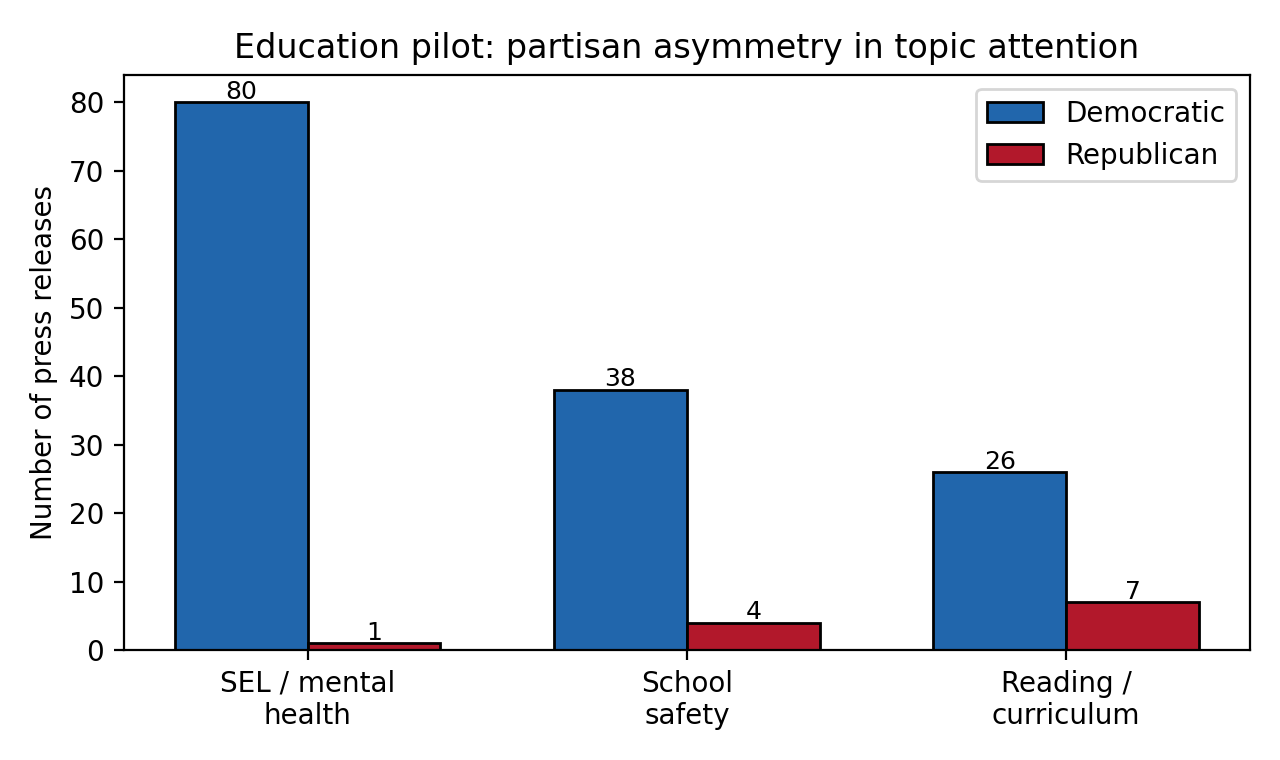
\includegraphics[width=0.6\textwidth]{fig_education.png}
\caption{Partisan asymmetry in education-policy attention (counts of press releases), illustrating that
the pipeline's front end generalizes beyond AI.}
\label{fig:edu}
\end{figure}

\section{Discussion}
\label{sec:discussion}

\paragraph{An LLM judge is necessary, not optional.} The most actionable methodological lesson is
negative: the standard discriminative tool for scientific claim verification---NLI entailment over
claim--evidence pairs \citep{wadden2020fact}---is not a safe stand-alone measure of whether science
supports a policy claim. It systematically labels genuine support as ``neutral,'' because an
abstract seldom restates a press-release claim in entailing language, and the resulting downward
bias is large enough to reverse a substantive conclusion (here, the apparent partisan gap in
evidence quality). A high-capacity generative judge, which reasons about whether the study's
findings \emph{bear on} the claim rather than whether the texts \emph{entail} one another, is
required to recover the right answer. This does not make NLI useless: it is cheap, fast, and
runs on every pair, which is exactly what a surrogate needs to be.

\paragraph{Validity without humans.} The combination that makes the pipeline both autonomous and
valid is surrogate-plus-judge-plus-PPI. Prediction-powered inference \citep{angelopoulos2023ppi}
and design-based supervised learning \citep{egami2023dsl} were developed to let researchers use
abundant imperfect labels alongside a small set of trusted labels; our contribution is to observe
that the ``trusted'' labels need not come from humans. A frontier LLM judge supplies
gold-equivalent labels at the scale of a few dozen to a few hundred items---enough to estimate and
correct the surrogate's bias---while the open-source NLI models supply the breadth. The
human research assistant, the traditional bottleneck and cost center of this kind of measurement,
is removed without sacrificing the inferential guarantees that justify the estimate.

\paragraph{Diagnose across methods, not within.} A practical corollary concerns how to know
whether an automated coder can be trusted. High agreement \emph{among} models of the same family
is reassuring but can be an illusion of correctness: our two NLI models agreed at $\kappa=0.65$
while sharing the very bias that distorted the estimate. The informative comparison is
\emph{across} paradigms---generative versus discriminative---and the alternative-annotator test
\citep{calderon2025alttest} formalizes when one may substitute for the other. We recommend reporting
cross-method agreement as a routine diagnostic in LLM-based measurement, precisely because
within-method agreement hid the problem here.

\paragraph{What we learn about AI policymaking.} Substantively, two findings stand out. First,
evidence use is higher than a naive automated reading suggests: most technical claims California
legislators make about AI are supported by the peer-reviewed literature our pipeline retrieves
(roughly 0.6--0.7 for both parties). Whatever one's priors about ``post-truth'' politics, in this
domain and at the level of discrete factual claims, legislators' assertions are largely backed by
science that exists and is mostly open-access. Second, the robust partisan asymmetry is in
\emph{engagement}, not \emph{accuracy}: Democrats talk about AI far more, and more intensively, than
Republicans, but once a competent judge is used the two parties' claims are supported at similar
rates. The headline ``Democrats use better evidence'' implied by the naive measure is an artifact of
the instrument, a cautionary tale for the rapidly growing practice of using off-the-shelf NLP to
score political text.

\paragraph{A template for computational social science.} Beyond this application, the design is a
reusable template: pair a cheap, scalable open-source classifier (the surrogate) with a small,
high-quality LLM-judge gold set, reconcile them with PPI/DSL, and validate by cross-method
agreement. It runs with no proprietary API and no human coders, which lowers both the cost and the
access barriers to large-scale, valid text measurement---and makes the whole analysis exactly
reproducible from released code and data.

% Limitations + Conclusion — TODO
\section{Limitations and Conclusion}
\label{sec:conclusion}


\section*{Acknowledgments}
Components of the data pipeline and the autonomous validation analysis were implemented and
executed with AI assistance (open-source NLI models and an in-context LLM judge); all design
decisions, interpretation, and claims are the authors'. Earlier pipeline development was
supported by NSF awards 2318460 and 2148215.

\bibliography{references}

\end{document}
